\documentclass[letterpaper,12pt]{article}

\usepackage{threeparttable}
\usepackage{geometry}
\geometry{letterpaper,tmargin=1in,bmargin=1in,lmargin=1.0in,rmargin=1.0in}
\usepackage[format=hang,font=normalsize,labelfont=bf]{caption}
\usepackage{amsmath}
\usepackage{multirow}
\usepackage{array}
\usepackage{delarray}
\usepackage{amssymb}
\usepackage{amsthm}
\usepackage{lscape}
\usepackage{natbib}
\usepackage{setspace}
\usepackage{float,color}
\usepackage[pdftex]{graphicx}
\usepackage{listings}
\lstset{basicstyle=\footnotesize\ttfamily, language=Python, showstringspaces=false}

\lstset{frame=single,
  language=Python,
  showstringspaces=false,
  columns=flexible,
  basicstyle={\small\ttfamily},
  numbers=none,
  breaklines=true,
  breakatwhitespace=true
  tabsize=3
}

\usepackage{pdfsync}
\usepackage{booktabs}
\usepackage{verbatim}
\usepackage{placeins}
\usepackage{geometry}
\usepackage{pdflscape}
\synctex=1
\usepackage{hyperref}
\hypersetup{colorlinks,linkcolor=red,urlcolor=blue,citecolor=red}
\usepackage{bm}


\theoremstyle{definition}
\newtheorem{theorem}{Theorem}
\newtheorem{acknowledgement}[theorem]{Acknowledgement}
\newtheorem{algorithm}[theorem]{Algorithm}
\newtheorem{axiom}[theorem]{Axiom}
\newtheorem{case}[theorem]{Case}
\newtheorem{claim}[theorem]{Claim}
\newtheorem{conclusion}[theorem]{Conclusion}
\newtheorem{condition}[theorem]{Condition}
\newtheorem{conjecture}[theorem]{Conjecture}
\newtheorem{corollary}[theorem]{Corollary}
\newtheorem{criterion}[theorem]{Criterion}
\newtheorem{definition}{Definition}  % Number definitions on their own
\newtheorem{derivation}{Derivation}  % Number derivations on their own
\newtheorem{example}[theorem]{Example}
\newtheorem{exercise}[theorem]{Exercise}
\newtheorem{lemma}[theorem]{Lemma}
\newtheorem{notation}[theorem]{Notation}
\newtheorem{problem}[theorem]{Problem}
\newtheorem{proposition}{Proposition}  % Number propositions on their own
\newtheorem*{proposition*}{Proposition}  % Non-numbered proposition
\newtheorem{remark}[theorem]{Remark}
\newtheorem{solution}[theorem]{Solution}
\newtheorem{summary}[theorem]{Summary}
\bibliographystyle{aer}
\newcommand\ve{\varepsilon}
%\renewcommand\theenumi{\roman{enumi}}
\newcommand\norm[1]{\left\lVert#1\right\rVert}

\begin{document}

\begin{titlepage}
\title{The Economic Costs of a Resurgence of Disease in South Africa}
\date{March 2025}
\author{\href{http://jasondebacker.com/}{Jason DeBacker}\thanks{University of South Carolina, Darla Moore School of Business, Department of Economics, \href{mailto:jason.debacker@moore.sc.edu}{jason.debacker@moore.sc.edu}. All Python code and documentation for the computational examples and analyses are available at \href{https://github.com/OpenSourceEcon/CostOfDisease}{https://github.com/OpenSourceEcon/CostOfDisease}.}\and \href{https://sites.google.com/site/rickecon}{Richard W. Evans}\thanks{\href{https://abundance.institute/}{Abundance Institute}, \href{mailto:rick@abundance.institute}{rick@abundance.institute}.}\and Marcelo T. LaFleur\thanks{United Nations Department of Economic Social Affairs}, \href{mailto:lafleurm@un.org}{lafleurm@un.org}.}
\maketitle
\vspace{-2mm}
\begin{abstract}
\small{Reductions in U.S. foreign aid are expected to have significant public health impacts.  We estimate the economic costs of these reductions in terms of lost health and productivity for South Africa.  We find that the reductions in foreign aid and expected significant increases in disease and premature death, will have very large and negative impacts on the South African economy.  In our preferred specification, the costs exceed XX trillion rand (about \$X trillion dollars) in net present value.}

\vspace{10mm}

\noindent\textit{keywords:}\: public health, demographics, general equilibrium, productivity, South Africa

\vspace{10mm}

\noindent\textit{JEL classification:} C68, E24, E37, I15, J11, J17, J24


\end{abstract}
\thispagestyle{empty}
\end{titlepage}


\begin{spacing}{1.5}

\pagenumbering{arabic}

\newpage

\section{Introduction}\label{SecIntro}

Background on aid to SA and their history of disease.  Cite \cite{KS2025} on costs.  Also cites Marcelo found on productivity effects.

\section{Methodology}\label{SecMethod}

We use the OG-ZAF model (cite it) to estimate the economic costs of a resurgence of disease in South Africa.  The model is a dynamic, general equilibrium model that includes a detailed representation of the South African economy, including its demographics, health, and productivity.  The model is calibrated to match the South African data and is used to simulate the economic impacts of a resurgence of disease in South Africa.

Give brief overview of model, but omit equations etc in main text.  Cite OG-Core as well as OG-ZAF (and footnote with links to docs for details).

Describe how we incorporate \cite{KS2025} into the model:

% figure
\begin{figure}[h]
    \caption{Mortality rates with and without aid}
    \centering
    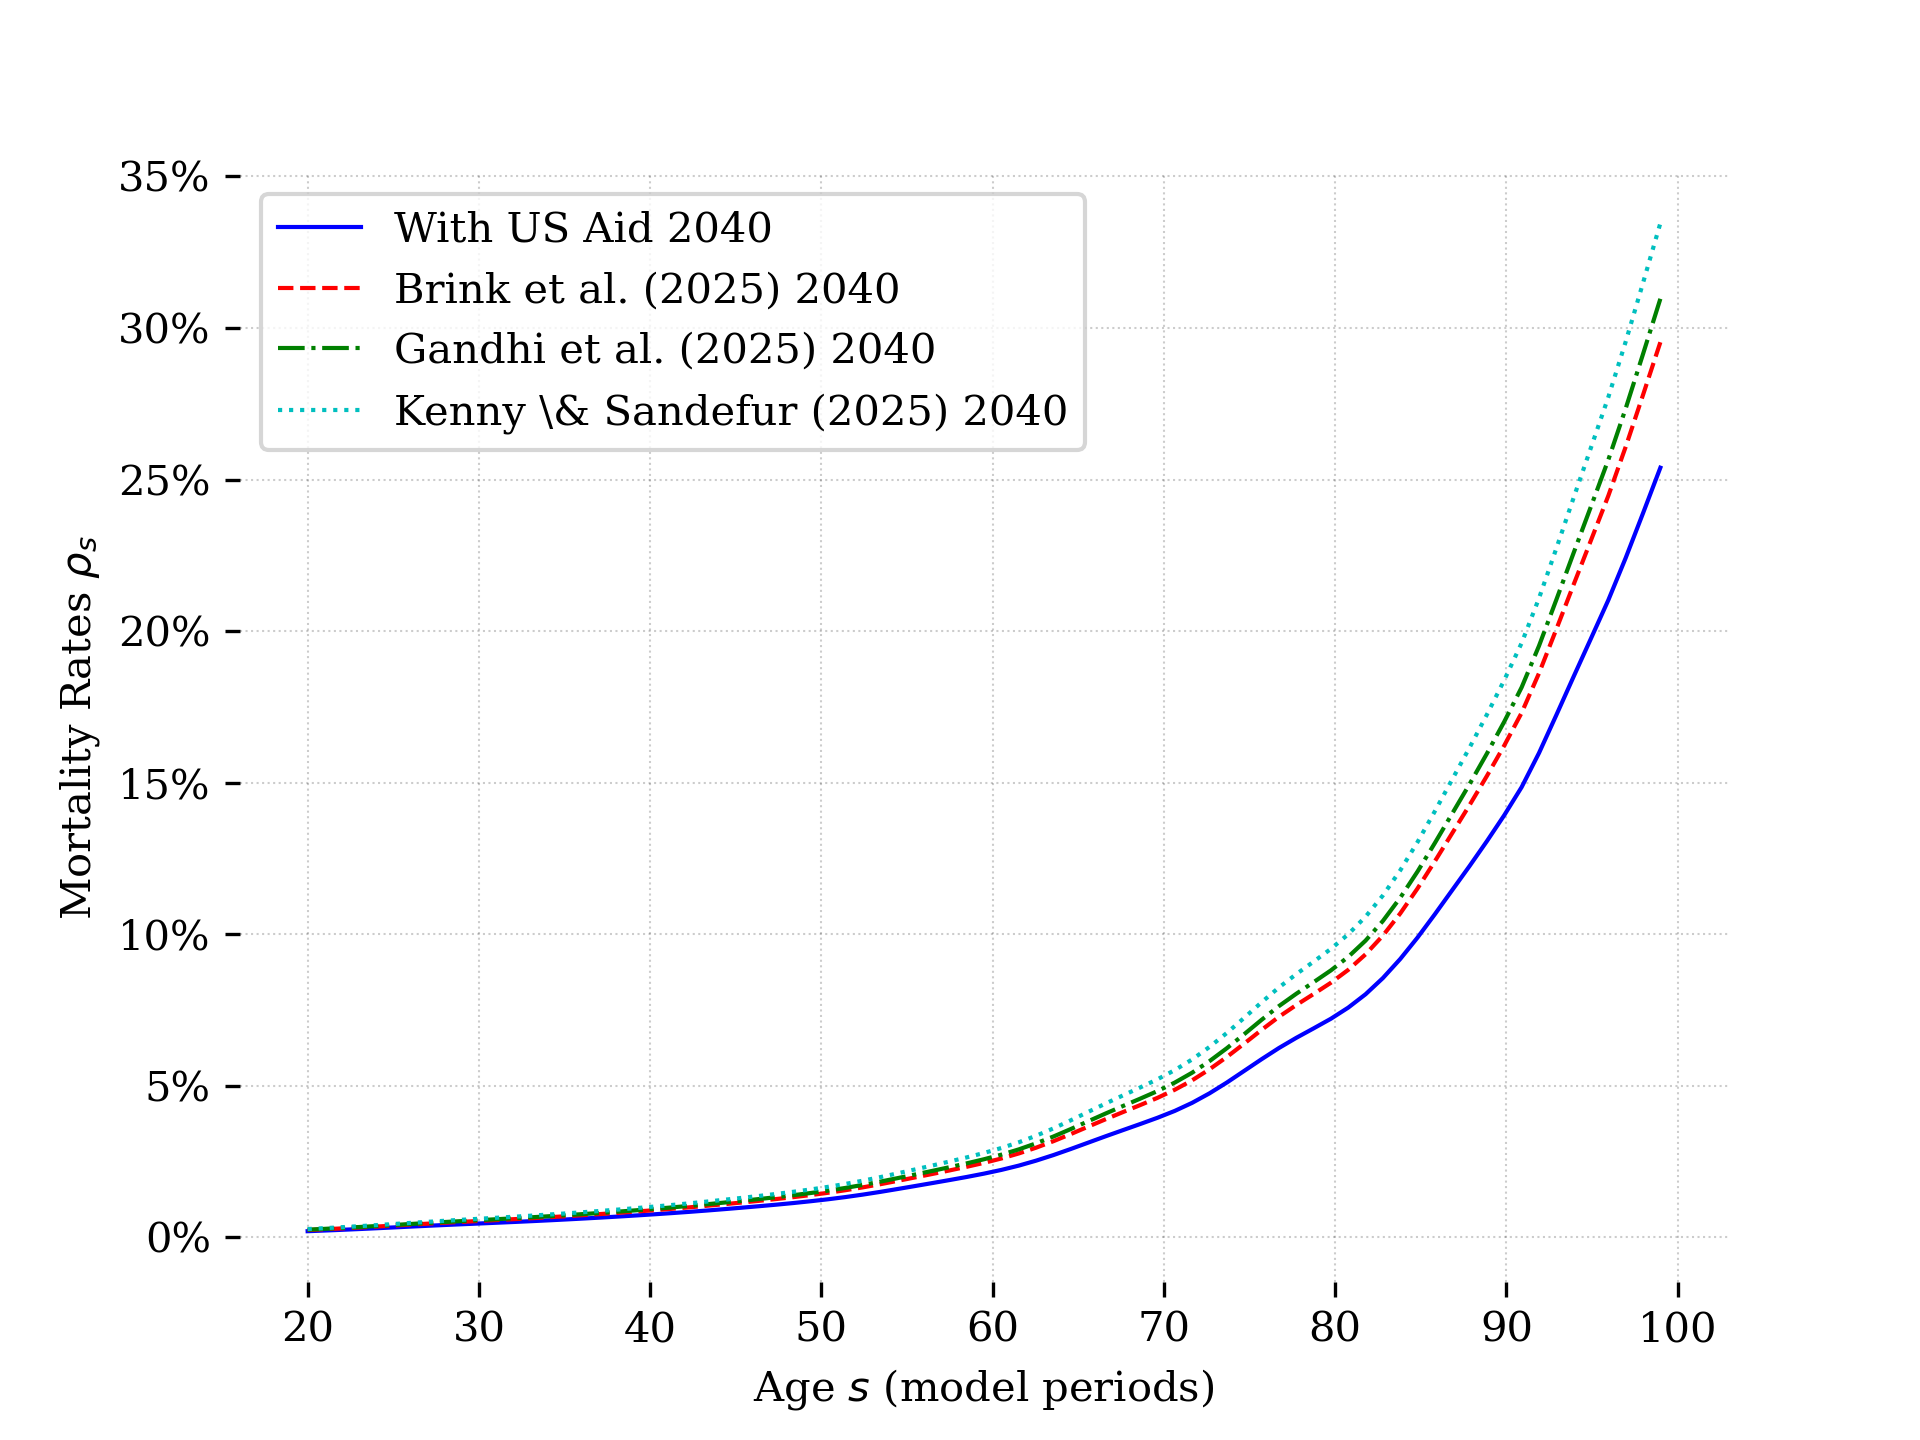
\includegraphics[scale=0.75]{./tables_figures/mortality_rates.png}
\end{figure}

The population distribution is affected by the changes in mortality rates:
\begin{figure}[h]
    \caption{The population distribution with and without aid}
    \centering
    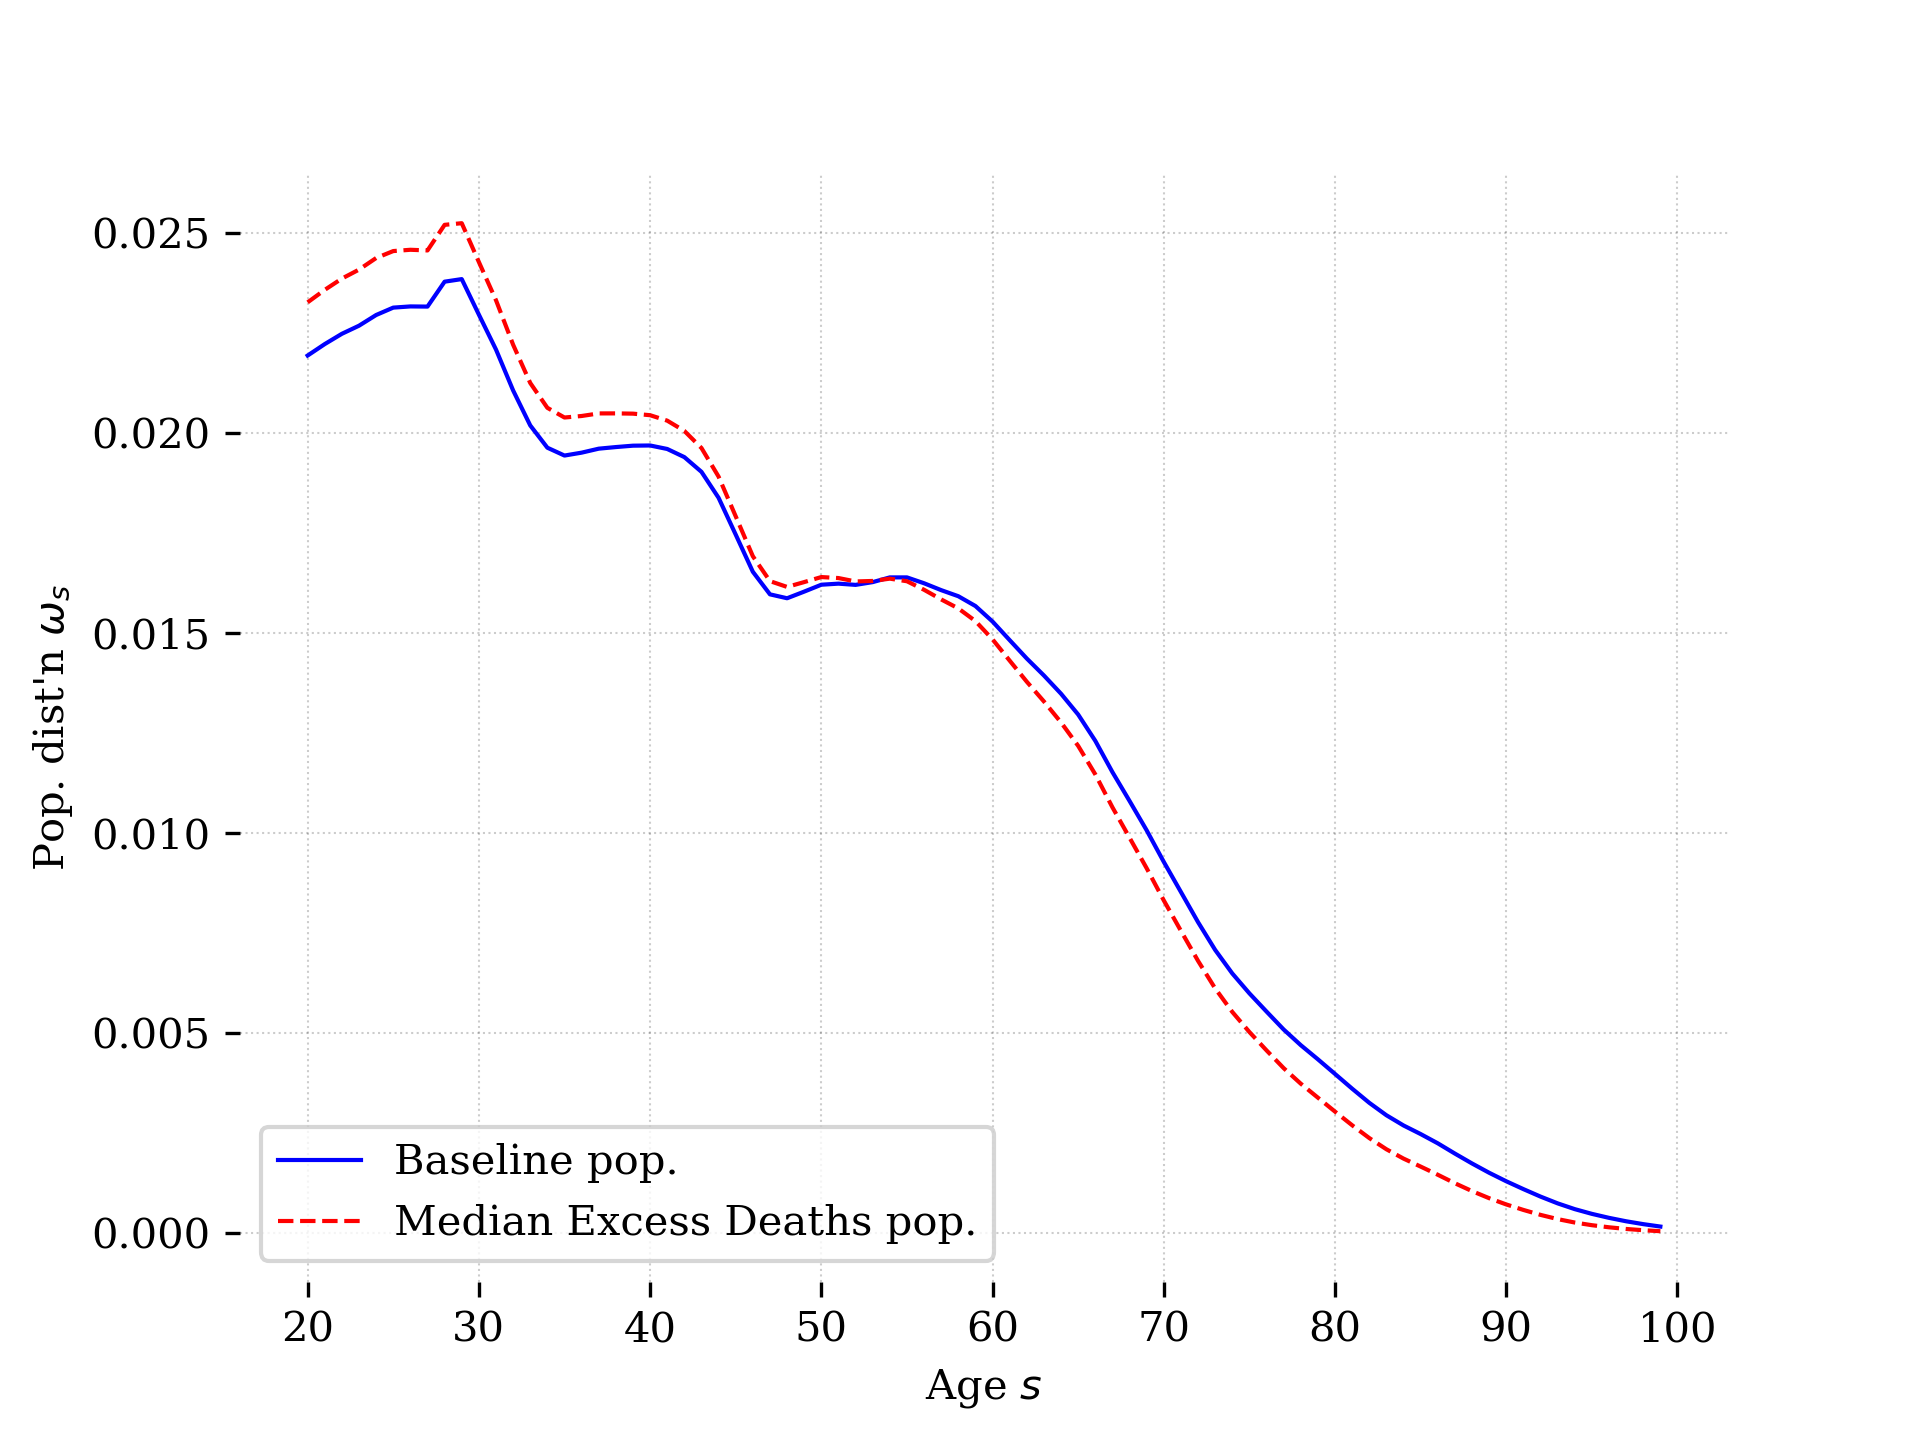
\includegraphics[scale=0.75]{./tables_figures/pop_dist_2050.png}
\end{figure}

TODO: create and add a figure here with cumulative deaths.

Describe how we incorporate productivity effects into the model (cite that research):

\begin{figure}[h]
    \caption{Labor productivity with and without aid}
    \centering
    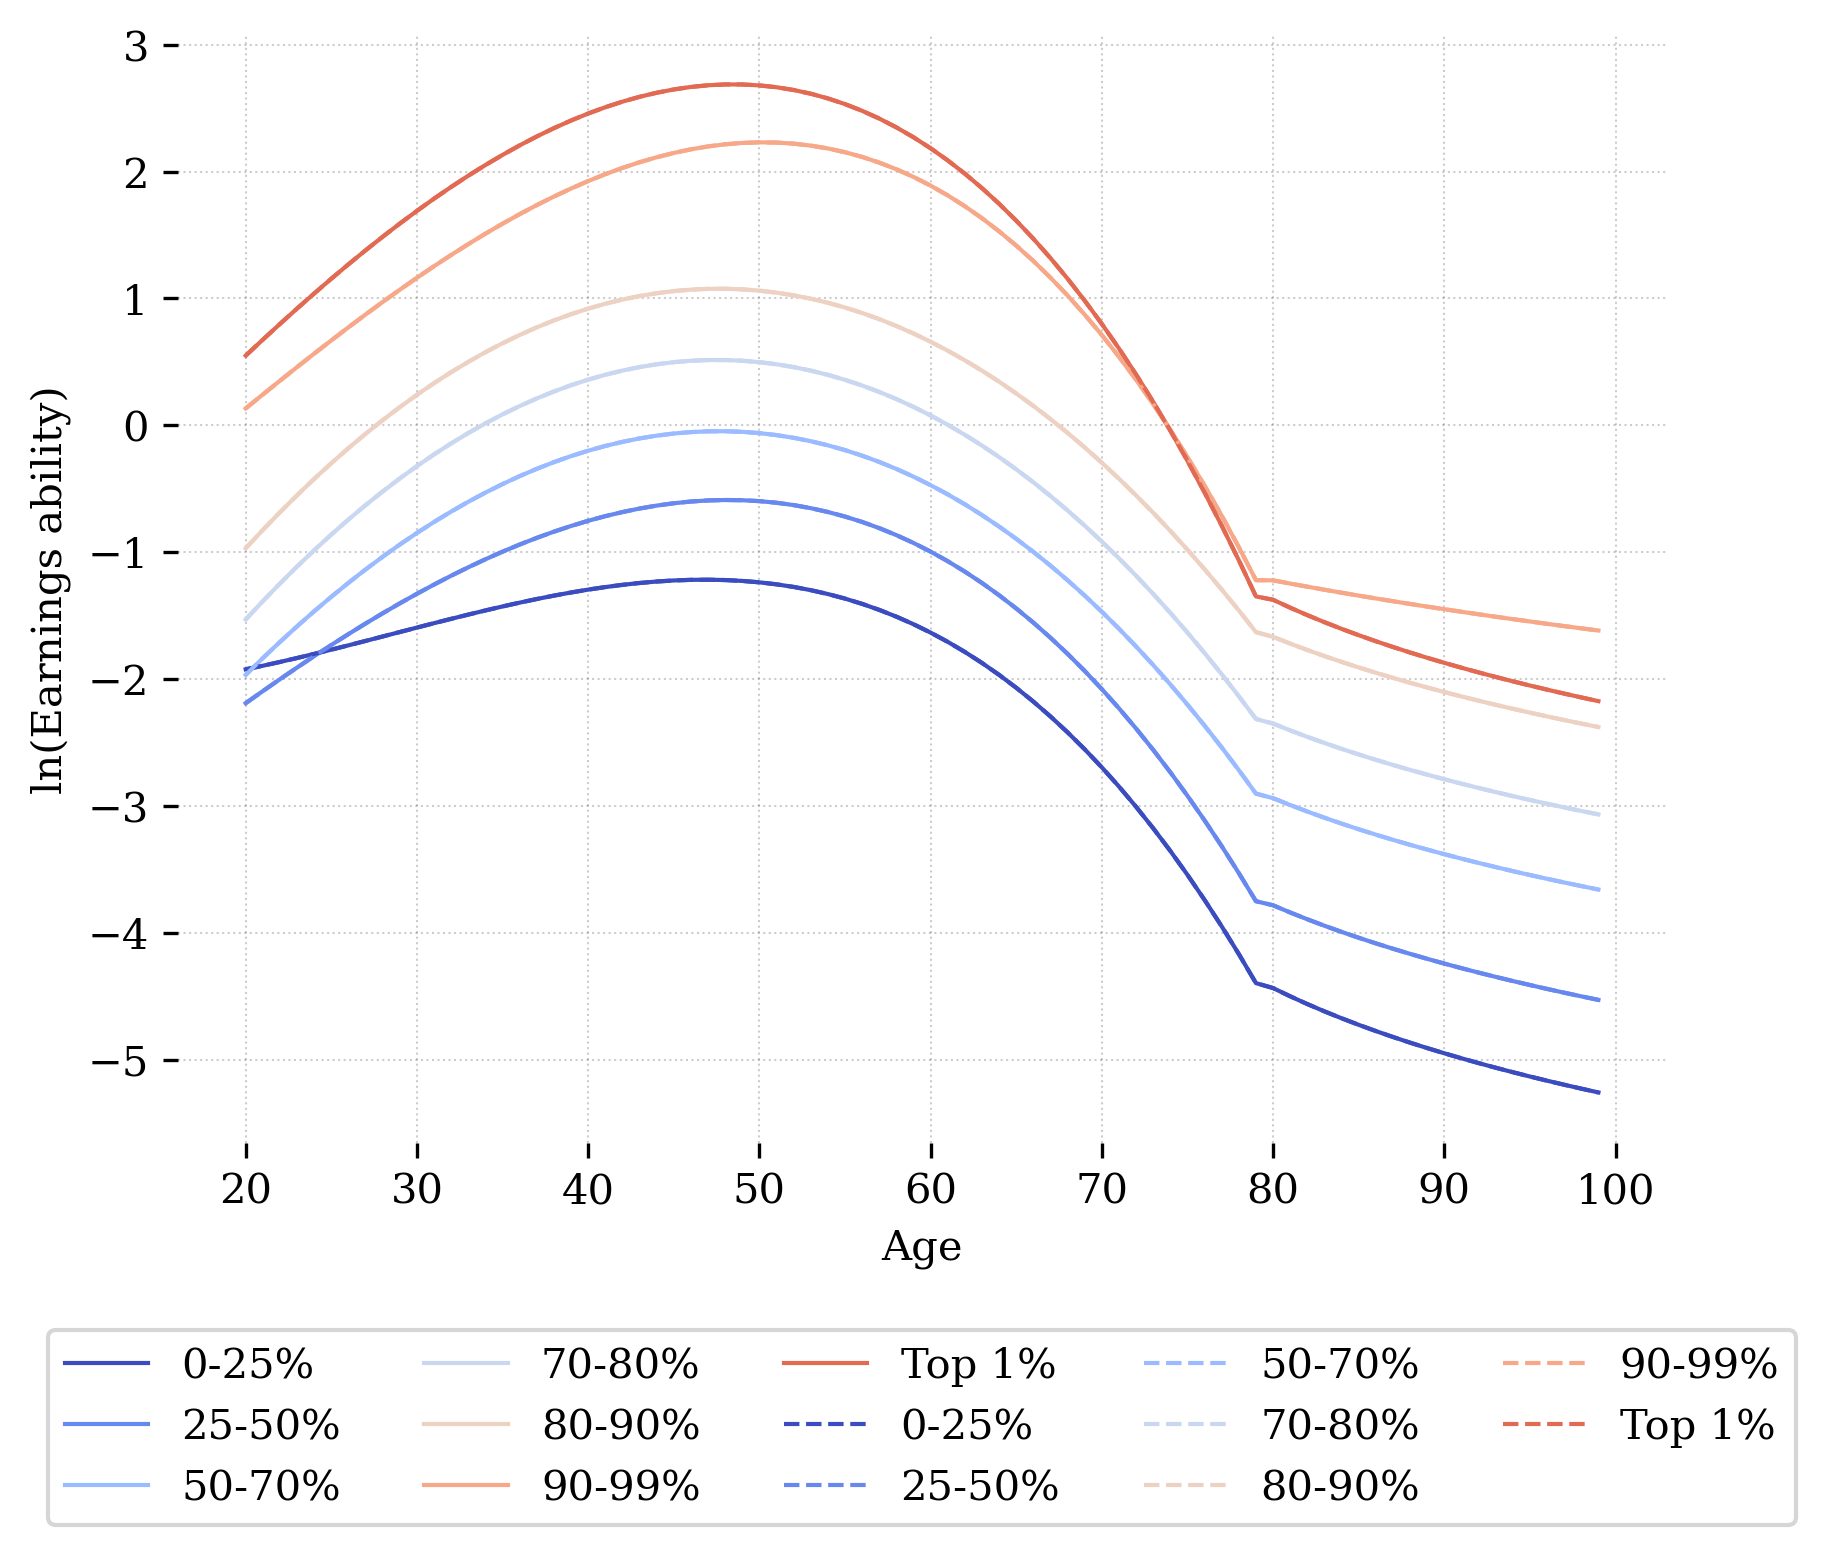
\includegraphics[scale=0.75]{./tables_figures/ability_profiles.png}
\end{figure}

\section{The Economics Costs of Disease}\label{SecResults}

We find that the economic costs of a resurgence of disease in South Africa are very large.  In our preferred specification, the costs exceed XX trillion rand (about \$X trillion dollars) in net present value.  The costs are driven by the large increases in mortality rates and the resulting reductions in labor productivity.

Put in tables and figures showing: Changes in GDP over first few years, NPV of effect, plot of cumulative deaths (or number of people).

Trillions per year. average over 20 years.
\begin{tabular}{lr}
\toprule
 & $\Delta$ GDP, Trillions \\
\midrule
Low Excess Deaths & -0.01 \\
Median Excess Deaths & -0.02 \\
High Excess Deaths & -0.02 \\
\bottomrule
\end{tabular}


NPV in trillions
\begin{tabular}{rlrrr}
\toprule
index & Discount Rate & Low Excess Deaths & Median Excess Deaths & High Excess Deaths \\
\midrule
0 & 2\% & -0.42 & -2.27 & -3.99 \\
1 & 4\% & -0.30 & -0.91 & -1.49 \\
2 & 6\% & -0.19 & -0.45 & -0.71 \\
\bottomrule
\end{tabular}


Have some robustness by looking at high and low values of the forecast of excess deaths/effects on productivity.

\section{Conclusion}\label{SecConc}

Sum up what we said.  Compare economic costs to the amount of aid that is at stake.

\end{spacing}
\newpage
\bibliography{disease.bib}


\end{document}